\newpage

\section{Bending lines to your will}

Another important part of a good layout is getting lines to be just the way you want them to be. In EA you can add and remove bending points which can be used
to control the appearance of a line.

\begin{stepbystep}
\item Hold down \texttt{Ctrl} and click on a line to create a bending point (\Cref{ea:bendLines}). You can now pull the bending point
and shift the line as you wish.
 
\begin{figure}[htbp]
\begin{center}
  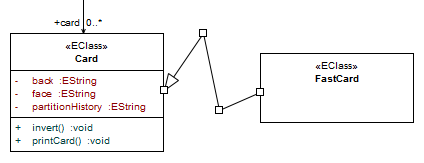
\includegraphics[width=0.8\textwidth]{../../org.moflon.doc.handbook.05_miscellaneous/1_grokkingEA/02_bendingLines/ea_bendingLines}
  \caption{Adding bending points to a line}   
  \label{ea:bendLines}
\end{center}
\end{figure}

\item You can create as many bending points as you wish, and you can \emph{remove} them by holding down \texttt{Ctrl} and clicking once
on the unwanted point.
\end{stepbystep}
